\documentclass{article}

% Camera-ready build. The `final' option removes line numbers and the
% "Submitted to" notice, prints the author block and shows the acknowledgments;
% `dblblindworkshop' selects the workshop footer required by the EconML call.
\usepackage[final,dblblindworkshop]{neurips_2026}
\workshoptitle{Economics for Machine Learning}

\usepackage[utf8]{inputenc}
\usepackage[T1]{fontenc}
\usepackage{hyperref}
\hypersetup{hidelinks}
\usepackage{url}
\usepackage{booktabs}
\usepackage{amsfonts}
\usepackage{amsmath}
\usepackage{amssymb}
\usepackage{amsthm}
\usepackage{nicefrac}
\usepackage{microtype}
\usepackage{xcolor}
\usepackage{graphicx}
\usepackage{enumitem}

\newtheorem{theorem}{Theorem}
\newtheorem{proposition}[theorem]{Proposition}
\newtheorem{corollary}[theorem]{Corollary}
\newtheorem{lemma}[theorem]{Lemma}
\newtheorem{assumption}{Assumption}
\theoremstyle{remark}
\newtheorem{finding}{Finding}

\DeclareMathOperator*{\esssup}{ess\,sup}
\newcommand{\Real}{\mathbb{R}}
\newcommand{\Prob}{\mathbb{P}}
\newcommand{\E}{\mathbb{E}}
\newcommand{\Yspace}{\mathcal{Y}}
\newcommand{\Bclass}{\mathcal{B}}
\newcommand{\indep}{\perp\!\!\!\perp}
\newcommand{\Wald}{\mathrm{Wald}}

\title{Instrument Validity as an Audit for Algorithmic Collective Action}

\author{%
  Yi Cui\\
  Department of Economics, University of North Carolina at Chapel Hill\\
  \texttt{cy15307130001@gmail.com}
}

\begin{document}

\maketitle

\begin{abstract}
Can a platform experiment detect coordinated users who invert a randomized
encouragement? Such users are defiers in the local average treatment effect
(LATE) framework and can distort the instrumental-variables (Wald) estimate
used for a launch decision. Under random assignment and exclusion, the
observable violation functional $V(P)$ sharply lower-bounds defier mass.
We restate this known bound, give a self-contained proof, and examine its
interpretation as an audit of collective action. The audit has no population
violation exactly when defier potential-outcome measures are dominated by
complier measures. With a positive first stage, exact mimicry is undetectable
and leaves Wald equal to LATE. By contrast, a near-mimicry example with $29\%$ defiers
has a complier effect of $1.0$ and Wald estimand $-0.45$, with $V(P)=0.0022$.
Simulations illustrate sensitivity to outcome laws, participation, and
exclusion. The audit detects violations of joint identifying assumptions;
interpreting them as coordination requires additional behavioral restrictions.
\end{abstract}

\section{Introduction}

Algorithmic collective action studies how a coordinated group of users can
change what a platform learns by acting on its training data: relabelling or
perturbing their own examples \citep{hardt2023aca}, reordering playlists
\citep{baumann2024playlists}, or competing with other collectives
\citep{karan2025two,battiloro2025multiple}.

We study a different lever: the randomized experiment that decides a launch.
Consider an encouragement design: a random subset of users
is shown a prompt to try a feature ($Z$), adoption is voluntary ($D$), and the
platform estimates an adoption effect on an engagement outcome ($Y$) using the
instrumental-variables (IV) estimate, the Wald ratio of the prompt's effect on
$Y$ to its effect on $D$. In a stylized example, a streaming service prompts half of
its listeners to try an algorithmic playlist, measures listening time, and
launches if the Wald estimate is positive. A fan community that wants the
opposite decision \citep[cf.][]{baumann2024playlists} cannot choose who is
prompted, but the prompt is visible, so members can condition on it: adopt when
not prompted, refuse when prompted. In the local average treatment effect
(LATE) framework \citep{imbens1994,angrist1996} they are \emph{defiers}, and
monotonicity, which rules defiers out, fails by design.

Under random assignment, exclusion, and no interference, coordinated
always-taking or never-taking cancels from the Wald numerator and denominator.
Coordinated compliance can change the complier population and its effect, but
preserves the LATE interpretation when all users are monotone. Defiance breaks
that interpretation by introducing a negatively weighted effect
(Lemma~\ref{lem:influence}). This motivates studying defiance without claiming
that it is the collective's optimal strategy.

We ask whether the experiment can audit such coordination from its own data,
without observing membership or communication. Random assignment, exclusion,
and monotonicity imply inequalities between observed outcome sub-distributions
\citep{balke1997,kitagawa2015,mourifie2017}, and the positive part of their
violation, $V(P)$ in \eqref{eq:V}, is a sharp lower bound on the defier share.
The bound is known. \citet{richardson2010binary} characterize every type
distribution compatible with binary $(Z,D,Y)$ data;
\citet{noack2021sensitivity} parameterizes monotonicity violations by the
defier share and by complier--defier outcome heterogeneity, the two quantities
we vary; \citet{kedagni2024robust} derive the identified set of the defier
share and robust bounds for complier and defier effects.
\citet{kowalski2019counting,christy2024counting} count defiers with
design-based likelihoods, and \citet{dechaisemartin2017,dahl2023} recover
effects under alternatives to monotonicity. We connect this identification
literature to collective action through a stylized platform decision problem.
Our contribution is the audit interpretation and an analysis of its limits;
we do not propose a new identification bound or a strategic equilibrium.

\paragraph{Contributions.}
\begin{itemize}[leftmargin=1.2em,itemsep=1pt,topsep=1pt]
\item Theorem~\ref{thm:audit} restates the sharp bound with a self-contained
proof. Section~\ref{sec:audit} connects it to equation (16) of
\citet{richardson2010binary}; Appendix~\ref{app:example} gives checkable examples.
\item Corollary~\ref{prop:stealth} expresses nondetectability as measure
domination. The known Wald decomposition (Lemma~\ref{lem:influence}) shows how
effect heterogeneity can change the estimated sign despite a small violation.
Finding~\ref{find:width} illustrates that the identified set widens along the
simulated mimicry path but need not along a separated path.
\item Simulations quantify power and robustness to the outcome law, the
partition, the degree of coordination, and exclusion; the audit and the first
stage detect different failures.
\end{itemize}

\section{Setup}\label{sec:setup}

A platform randomizes an encouragement $Z\in\{0,1\}$, with $0<\Prob(Z=1)<1$,
and observes take-up $D\in\{0,1\}$ and an outcome $Y$ in a Polish space $\Yspace$.
We assume consistency, $D=D(Z)$ and $Y=Y(Z,D)$, and no interference between
users. Principal strata are $T=(D(0),D(1))$: $a=(1,1)$ always-takers,
$n=(0,0)$ never-takers, $c=(0,1)$ compliers, and $f=(1,0)$ defiers. Except in
the exclusion-sensitivity simulations, we maintain
\begin{assumption}[Random assignment]\label{a1} $Z\indep\big(Y(\cdot,\cdot),D(\cdot)\big)$. \end{assumption}
\begin{assumption}[Exclusion]\label{a2} $Y(z,d)=Y(d)$ almost surely. \end{assumption}
We do \emph{not} impose monotonicity, $\Prob(T=f)=0$, equivalently a
threshold-crossing model of take-up \citep{vytlacil2002}.

\paragraph{Terminology.} For treatment-effect statements, outcomes are real and
integrable and $\Prob(T=c)>0$. The LATE is
$\tau_c=\E[Y(1)-Y(0)\mid T=c]$. The Wald estimand is the reduced form
$\E[Y\mid Z{=}1]-\E[Y\mid Z{=}0]$ divided by the nonzero first stage
$\Prob(D{=}1\mid Z{=}1)-\Prob(D{=}1\mid Z{=}0)$; under
Assumptions~\ref{a1}--\ref{a2} and monotonicity it equals $\tau_c$.
A data-generating process (DGP) specifies the type shares and potential-outcome
laws. Write $\mu_t^{(d)}(B)=\Prob(T=t,Y(d)\in B)$ for their sub-measures.

\paragraph{The collective.} In the baseline recruitment model an active share
$\alpha$ inverts the encouragement and every non-member is monotone, so
$\Prob(T=f)=\alpha$. For positive stratum shares, \emph{exact mimicry} means
$\mu_f^{(d)}/\alpha=\mu_c^{(d)}/\Prob(T=c)$ for $d=0,1$.
In the simulations, $\mathrm{sep}$ shifts the untreated defier mean relative
to compliers, in baseline standard deviations; the treated mean differs by
$\mathrm{sep}+\tau_f-\tau_c$. Exact mimicry requires both
$\mathrm{sep}=0$ and $\tau_f=\tau_c$ in the common-scale family.

\paragraph{Observables.} Let $m_{dz}(B)=\Prob(Y\in B,D{=}d\mid Z{=}z)$ be the four observed sub-distributions. Under Assumptions~\ref{a1}--\ref{a2},
\begin{align}
m_{11}&=\mu_a^{(1)}+\mu_c^{(1)}, & m_{10}&=\mu_a^{(1)}+\mu_f^{(1)}, &
m_{00}&=\mu_n^{(0)}+\mu_c^{(0)}, & m_{01}&=\mu_n^{(0)}+\mu_f^{(0)}.\notag
\end{align}
Always-takers and never-takers appear in both members of each pair and cancel in the differences
\begin{equation}\label{eq:S}
S_1:=m_{10}-m_{11}=\mu_f^{(1)}-\mu_c^{(1)},\qquad
S_0:=m_{01}-m_{00}=\mu_f^{(0)}-\mu_c^{(0)},
\end{equation}
With $S=S_+-S_-$ the Jordan decomposition, define the \textbf{violation functional}
\begin{equation}\label{eq:V}
V(P):=\max\Big\{\,\sup_{B}S_1(B),\ \sup_{B}S_0(B)\Big\}=\max\big\{S_{1+}(\Yspace),\,S_{0+}(\Yspace)\big\}.
\end{equation}
The suprema range over Borel sets. $V(P)$ is the largest excess probability
mass prohibited by monotonicity. Under monotonicity,
$S_d=-\mu_c^{(d)}\le0$ for $d=0,1$, so $V(P)=0$; these are the
testable LATE inequalities \citep{kitagawa2015,mourifie2017}.

\section{The audit}\label{sec:audit}

\begin{theorem}[Sharp lower bound on defier mass]\label{thm:audit}
Let $P$ be the distribution of $(Z,D,Y)$ under some model satisfying Assumptions~\ref{a1}--\ref{a2}. Then
\[
\Prob(T=f)\ \ge\ V(P),
\]
and the bound is sharp: a model satisfying Assumptions~\ref{a1}--\ref{a2} induces $P$ with $\Prob(T=f)=V(P)$.
\end{theorem}

Theorem~\ref{thm:audit} is the lower endpoint of the identified set for the
defier share in \citet[Prop.~1]{kedagni2024robust}, who credit
\citet{richardson2010binary} for binary outcomes and
\citet[Prop.~1, eq.~(15)]{noack2021sensitivity} for the general case. The lower bound is immediate
from \eqref{eq:S}: $S_1(B)\le\mu_f^{(1)}(B)\le\Prob(T=f)$ for every $B$.
Appendix~\ref{app:proof} gives a self-contained attainment proof by Jordan
decomposition and a linear-program check over $30$ discretized models that
agrees with $V(P)$ to within $8.3\times10^{-8}$.

\paragraph{Binary outcomes.} For $\Yspace=\{0,1\}$, equation (16) of
\citet{richardson2010binary} writes $\pi_{DE}=\Prob(D{=}1\mid Z{=}0)-\pi_{AT}$
with $\pi_{AT}\le u_{\pi_{AT}}$. Subtracting the six terms of $u_{\pi_{AT}}$
from $\Prob(D{=}1\mid Z{=}0)$ gives $0$, $S_1(\Yspace)$, $S_1(\{0\})$,
$S_1(\{1\})$, $S_0(\{0\})$, and $S_0(\{1\})$, so their lower bound on
$\pi_{DE}$ is $V(P)$ with $B$ over subsets of $\{0,1\}$, and
Theorem~\ref{thm:audit} is the general-outcome form. Appendix~\ref{app:example}
works an example with $\alpha=0.10$ and $V(P)=0.03$.

\paragraph{Using the bound.} The population quantity $V(P)$ lower-bounds defier
mass. A sample rejection flags incompatibility with the joint assumptions;
neither rejection nor the plug-in estimate supplies a numerical confidence
bound. A platform can investigate exclusion and report sensitivity to defiers
before using Wald for a launch decision. Our identified sets are population
calculations, not confidence regions.

\section{Limits of the audit}\label{sec:limits}

\begin{corollary}[When violations are undetectable]\label{prop:stealth}
$V(P)=0$ if and only if $\mu_f^{(1)}\le\mu_c^{(1)}$ and $\mu_f^{(0)}\le\mu_c^{(0)}$ as measures. In particular, exact mimicry is undetectable by these inequalities whenever $\alpha\le\Prob(T=c)$.
\end{corollary}

This follows from \eqref{eq:V}: $S_{1+}(\Yspace)=0$ if and only if $S_1\le0$.
The audit also does not distinguish coordinated from idiosyncratic defiance,
and a rejection is evidence against the joint of Assumptions~\ref{a1}--\ref{a2}
and monotonicity, so attributing it to defiers requires exclusion
(Appendix~\ref{app:robust}). For $\alpha>0$, let
$\tau_f=\E[Y(1)-Y(0)\mid T=f]$.

\begin{lemma}[Influence; \citealp{angrist1996,noack2021sensitivity}]\label{lem:influence}
If $0<\alpha=\Prob(T=f)<\Prob(T=c)$, the Wald estimand equals
$\big(\Prob(T{=}c)\tau_c-\alpha\tau_f\big)/\big(\Prob(T{=}c)-\alpha\big)$, so
$|\Wald-\tau_c|=\alpha\,|\tau_c-\tau_f|/\big(\Prob(T{=}c)-\alpha\big)$, which
diverges as $\alpha\uparrow\Prob(T=c)$ with a fixed nonzero effect contrast.
\end{lemma}

The reduced form is $\Prob(T=c)\tau_c-\alpha\tau_f$ and the first stage
$\Prob(T=c)-\alpha$. With a nonzero first stage, exact mimicry implies
$\tau_f=\tau_c$ and no distortion.
Small violations can nevertheless accompany substantial distortion: with
$\alpha=0.29$, $\Prob(T=c)=0.30$, $\tau_f=1.05$,
$\tau_c=1$, and the Gaussian outcomes of Section~\ref{sec:exp} with
$\mathrm{sep}=0$, the platform
reports $\Wald=-0.45$ while $V(P)=0.0022$.

\begin{finding}[Information loss in the discretized simulation]\label{find:width}
For midpoint-coded outcomes $Q(Y)$, the sharp identified-set width for
$\tau_c^Q=\E[Q(Y(1))-Q(Y(0))\mid T=c]$ need not be monotone in $\alpha$.
The linear-fractional program in Appendix~\ref{app:sim} gives an increase
from $1.30$ to $6.30$ as $\alpha$ moves from $0$ to $0.29$ under exact mimicry,
but a non-monotone path from $1.30$ to $1.31$ for $\mathrm{sep}=3$
(Figure~\ref{fig:main}c).
\end{finding}

These sets allow all type shares and outcome laws compatible with the
discretized observables; neither $\alpha$ nor mimicry is imposed on candidate
models. The contrast between paths in Figure~\ref{fig:main}c is numerical,
not a general ordering of detectability and information loss.

\section{Experiments}\label{sec:exp}

\paragraph{Design.} Outcomes are Gaussian with unit variance: compliers have
$Y(0)\sim\mathcal N(0,1)$ and $Y(1)\sim\mathcal N(\tau_c,1)$ with $\tau_c=1$,
collective members are shifted by $\mathrm{sep}$ with effect $\tau_f$, and
$\Prob(T=c)=0.30$, $\Prob(T=a)=0.25$, $\Prob(T=f)=\alpha$
(Appendix~\ref{app:sim}). Rejection rates use $400$ replications (Monte Carlo
standard error at most $0.025$) of the studentized test of the $24$ cellwise
inequalities on $12$ cells of $[-6,9]$ at level $0.05$ (Appendix~\ref{app:sim});
the histogram plug-in estimates the partition-restricted bound, which is no
larger than $V(P)$, with upward sampling bias.

\begin{figure}[t]
\centering
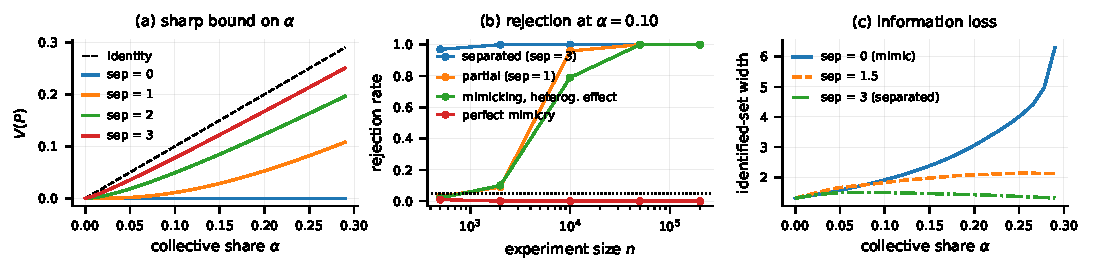
\includegraphics[width=\linewidth]{figs/fig_main.pdf}
\caption{(a) $V(P)$ against $\alpha$ at four separations. (b) Rejection rates
at $\alpha=0.10$; mimicry lies inside the composite null, so rejection can be
below $0.05$. (c) Width of the identified set for $\tau_c^Q$
(Finding~\ref{find:width}).}
\label{fig:main}
\end{figure}

\paragraph{Separation and mimicry.} Under $\mathrm{sep}=3$, $\alpha=0.01$ gives
$V(P)=0.005$ and rejection rates $0.09$, $0.99$, and $1.00$ at
$n=2{,}000$, $10{,}000$, and $50{,}000$. At $n=2{,}000$, the rate is $0.65$
for $\alpha=0.02$ and $1.00$ for $\alpha=0.05$. At $\alpha=0.10$
(Figure~\ref{fig:main}b), $\mathrm{sep}=3$ is detected with rate $0.96$ at
$n=500$, and $\mathrm{sep}=1$ reaches $0.94$ at $n=10{,}000$.
Exact mimicry with $\alpha=0.10<\Prob(T=c)=0.30$ is rejected at most $0.01$
at each tested size; Appendix~\ref{app:robust} separately checks a boundary null.

\paragraph{The first stage is complementary.} The sign-flipping configuration
is rejected in $18\%$ of samples at $n=200{,}000$. Its first stage of $0.01$
amplifies effect heterogeneity; assessing instrument strength also requires
sampling precision. At $\alpha=0.05$ with $\tau_f=3$, Wald is $0.60$ against
$\tau_c=1$ with $V(P)=0.018$ and a larger first stage of $0.25$.

\paragraph{Robustness.} Appendix~\ref{app:robust} varies outcome laws, partitions,
participation, idiosyncratic defiers, and exclusion. Rejection is at most
$0.01$ under the strict-domination mimicry designs; power depends on the outcome law and
partition. Passive compliers can mask active defiers. A direct effect of $0.3$
standard deviations with no defiers is rejected in $93\%$ of samples at
$n=50{,}000$, illustrating the need to assess exclusion.

\section{Discussion}\label{sec:disc}

The audit bounds defier mass; its coordination interpretation requires the
recruitment model. Strategies are taken as given. Modeling a learning system
and a collective--auditor equilibrium remains future work, requiring explicit
objectives, timing, and costs. Appendices~\ref{app:limits}--\ref{app:frontier}
discuss limitations, dual use, and simulated detectability--influence pairs.

\clearpage
% \begin{ack}
% I thank the three anonymous EconML reviewers for comments that improved the
% positioning and presentation of this paper, in particular for the pointers to
% \citet{richardson2010binary} and \citet{noack2021sensitivity}. Code
% reproducing every number and figure is distributed with the paper.
% \end{ack}

\bibliographystyle{plainnat}
\bibliography{refs}

\appendix

\section{Proof of Theorem~\ref{thm:audit}}\label{app:proof}

Fix $P$ in the image of the model, i.e.\ generated by some $\mu^\star=(\mu_a^{(1)},\mu_n^{(0)},\mu_c^{(1)},\mu_c^{(0)},\mu_f^{(1)},\mu_f^{(0)})$ satisfying Assumptions~\ref{a1}--\ref{a2}.

\paragraph{Lower bound.} By \eqref{eq:S}, for any Borel $B$, $S_1(B)=\mu_f^{(1)}(B)-\mu_c^{(1)}(B)\le\mu_f^{(1)}(B)\le\Prob(T=f)$, so $S_{1+}(\Yspace)\le\Prob(T=f)$. The same argument applies to $S_0$, hence $V(P)\le\Prob(T=f)=\alpha$ in the baseline recruitment model.

\paragraph{Attainment.} Let $\varphi:=V(P)$ and recall $\delta=\Prob(T=f)-\Prob(T=c)=m_{10}(\Yspace)-m_{11}(\Yspace)=m_{01}(\Yspace)-m_{00}(\Yspace)$ is identified. We construct a model inducing $P$ with $\Prob(T=f)=\varphi$.

For $d=0,1$, let $v_d=S_{d+}(\Yspace)$. The Jordan decomposition gives
$S_{d-}(\Yspace)=v_d-\delta$ and $\varphi\ge v_d\ge\max\{0,\delta\}$.
Define the nonnegative common parts
\[
A_1=m_{10}-S_{1+}=m_{11}-S_{1-},\qquad
A_0=m_{01}-S_{0+}=m_{00}-S_{0-}.
\]
Nonnegativity follows from $(m_{10}-m_{11})_+\le m_{10}$ and its analogues.
Choose sub-measures $0\le R_d\le A_d$ of mass $\varphi-v_d$ and set
\[
\mu_f^{(d)}=S_{d+}+R_d,\qquad
\mu_c^{(d)}=S_{d-}+R_d,\qquad
\mu_a^{(1)}=A_1-R_1,\qquad \mu_n^{(0)}=A_0-R_0.
\]
Such $R_1$ exists precisely when $\varphi\le m_{10}(\Yspace)$, and $R_0$
exists when $\varphi\le m_{01}(\Yspace)$: take a suitable scalar multiple
of $A_d$ (or zero when its mass is zero). Both inequalities hold because some
valid generating model exists and its defier share lies between $\varphi$ and
$\min\{m_{10}(\Yspace),m_{01}(\Yspace)\}$. This uses feasibility of $P$,
not the conclusion to be proved.

The constructed shares are
\[
(\Prob(T=f),\Prob(T=c),\Prob(T=a),\Prob(T=n))
=(\varphi,\varphi-\delta,m_{10}(\Yspace)-\varphi,m_{01}(\Yspace)-\varphi).
\]
They are nonnegative and sum to
$m_{10}(\Yspace)+m_{01}(\Yspace)-\delta=1$.
Within each positive-mass complier or defier stratum, couple the normalized
potential-outcome marginals arbitrarily, for example independently. Assign
arbitrary unobserved $Y(0)$ for always-takers and $Y(1)$ for never-takers.
Draw $Z$ independently with its observed assignment probability and impose
consistency and exclusion. The resulting model induces $P$ and has defier
share $\varphi=V(P)$. \hfill$\square$

\paragraph{Numerical check.} Independently of the proof, we minimized $\Prob(T=f)$ by linear programming over a $14$-cell discretized feasible set (four equalities per outcome cell, equal stratum mass across $d$, total mass one, nonnegativity) and compared the minimum with the cellwise $V(P)$ across $30$ data-generating processes spanning $\alpha\in\{0.02,0.05,0.10,0.20,0.29\}$, separations $\{0,1,2.5\}$ and $\tau_f\in\{1,2\}$. The maximum absolute discrepancy was $8.3\times10^{-8}$, at linear-program tolerance.

\section{A worked binary example}\label{app:example}

Let $\Yspace=\{0,1\}$ with shares $\Prob(T=a)=0.25$, $\Prob(T=n)=0.35$, $\Prob(T=c)=0.30$, and $\alpha=\Prob(T=f)=0.10$. Write $p_t(d)=\Prob(Y(d){=}1\mid T{=}t)$ and take $p_a(1)=0.5$, $p_n(0)=0.6$, $p_c(0)=0.4$, $p_c(1)=0.2$, $p_f(0)=0.4$, and $p_f(1)=0.9$, so the collective mimics compliers under $d=0$ and is separated under $d=1$. The observed cells, listed as $(y{=}0,\,y{=}1)$, are
\begin{gather*}
m_{11}=(0.365,\,0.185),\qquad m_{10}=(0.135,\,0.215),\\
m_{00}=(0.320,\,0.330),\qquad m_{01}=(0.200,\,0.250);
\end{gather*}
for instance $m_{11}(\{1\})=0.25\times0.5+0.30\times0.2=0.185$ and $m_{10}(\{1\})=0.25\times0.5+0.10\times0.9=0.215$. Hence
\begin{gather*}
S_1(\{1\})=0.03,\quad S_1(\{0\})=-0.23,\quad S_0(\{1\})=-0.08,\quad S_0(\{0\})=-0.12,\\
S_1(\Yspace)=S_0(\Yspace)=-0.20,
\end{gather*}
and $V(P)=0.03$. At the population level, these observables require at least $3\%$ defiers although the generating share is $10\%$. The additional $7$ percentage points are not required to rationalize the data; this statement does not identify particular users. The attaining model of Theorem~\ref{thm:audit} has shares $(f,c,a,n)=(0.03,0.23,0.32,0.42)$, and the linear program of Appendix~\ref{app:proof} returns the same minimum. The Wald estimand is $(0.435-0.545)/0.20=-0.55$ while $\tau_c=-0.2$ and $\tau_f=0.5$, matching Lemma~\ref{lem:influence}: $(0.30\times(-0.2)-0.10\times0.5)/0.20=-0.55$. In the notation of \citet{richardson2010binary}, $p(x{=}1\mid z{=}0)=0.35$ and the six terms of $u_{\pi_{AT}}$ are $0.35$, $0.55$, $0.43$, $0.47$, $0.32$, and $0.58$, so $\pi_{DE}\ge0.35-0.32=0.03$, again $V(P)$. The script \texttt{robustness.py} reproduces every number.

\paragraph{Domination without exact mimicry.}
Keep the same shares and always-/never-taker laws, but set
$(p_c(0),p_c(1))=(0.4,0.6)$ and $(p_f(0),p_f(1))=(0,1)$.
Then $S_0=(-0.08,-0.12)$ and $S_1=(-0.12,-0.08)$, so $V(P)=0$ although
$\tau_c=0.2$ and $\tau_f=1$. The first stage is $0.2$ and
$\Wald=(0.30\times0.2-0.10\times1)/0.2=-0.2$.
Thus measure domination can hide a sign reversal, whereas exact mimicry
cannot. The binary example is also checked in \texttt{robustness.py}.

\section{Robustness of the audit}\label{app:robust}

\begin{table}[h]
\centering
\caption{Rejection rates of the moment-inequality test when the data depart from the Gaussian model of Section~\ref{sec:exp}. FS is the first stage. Unless stated, $\alpha=0.10$, $\Prob(T=c)=0.30$, $\Prob(T=a)=0.25$, $\tau_c=\tau_f=1$, and $12$ cells; $\Prob(T{=}f)$ is total defier mass. Participation rows recruit $0.10$ and split it into active defiers and passive compliers ($0.08/0.02$ and $0.05/0.05$). Rejection rates use $400$ replications (Monte Carlo standard error at most $0.025$) and seeds different from Figure~\ref{fig:main}.}
\label{tab:robust}
\footnotesize
\setlength{\tabcolsep}{3.5pt}
\resizebox{\textwidth}{!}{% Auto-generated by code/robustness.py -- do not edit by hand.
\begin{tabular}{@{}llrrrrrrr@{}}
\toprule
Outcome law & Collective & $\Prob(T{=}f)$ & $V(P)$ & FS & Wald & $n{=}2{,}000$ & $n{=}10{,}000$ & $n{=}50{,}000$\\
\midrule
Gaussian & sep $=1$ (baseline) & 0.10 & 0.011 & 0.20 & 1.00 & 0.20 & 0.95 & 1.00\\
Gaussian & exact mimicry & 0.10 & 0.000 & 0.20 & 1.00 & 0.00 & 0.00 & 0.01\\
Student-$t_3$ & sep $=1$ & 0.10 & 0.024 & 0.20 & 1.00 & 0.19 & 0.89 & 1.00\\
Student-$t_3$ & exact mimicry & 0.10 & 0.000 & 0.20 & 1.00 & 0.00 & 0.00 & 0.00\\
log-normal & sep $=1$ & 0.10 & 0.009 & 0.20 & 1.00 & 0.05 & 0.17 & 0.88\\
log-normal & exact mimicry & 0.10 & 0.000 & 0.20 & 1.00 & 0.00 & 0.00 & 0.00\\
binary & App.~\ref{app:example} example & 0.10 & 0.030 & 0.20 & -0.55 & 0.30 & 0.92 & 1.00\\
binary & exact mimicry & 0.10 & 0.000 & 0.20 & -0.20 & 0.00 & 0.00 & 0.00\\
Gaussian & equal means, $\sigma_f=2$ & 0.10 & 0.019 & 0.20 & 1.00 & 0.28 & 1.00 & 1.00\\
Gaussian & sep $=1$, $80\%$ participation & 0.08 & 0.003 & 0.24 & 1.00 & 0.01 & 0.15 & 0.83\\
Gaussian & sep $=1$, $50\%$ participation & 0.05 & 0.000 & 0.30 & 1.00 & 0.00 & 0.00 & 0.00\\
Gaussian & sep $=3$, $\alpha=0.05$ & 0.05 & 0.035 & 0.25 & 1.00 & 1.00 & 1.00 & 1.00\\
Gaussian & sep $=3$, $\alpha=0.05$, $+0.05$ idiosyncratic & 0.10 & 0.036 & 0.20 & 1.00 & 1.00 & 1.00 & 1.00\\
Gaussian & none; direct effect $0.1$ & 0.00 & 0.000 & 0.30 & 1.33 & 0.00 & 0.00 & 0.01\\
Gaussian & none; direct effect $0.3$ & 0.00 & 0.005 & 0.30 & 2.00 & 0.02 & 0.16 & 0.93\\
\bottomrule
\end{tabular}
}
\end{table}

Table~\ref{tab:robust} re-runs the test under departures from the Gaussian model. Continuous outcome laws are standardized to mean zero and unit variance before the location shifts of Appendix~\ref{app:sim} are applied, so $\mathrm{sep}$ is measured in standard deviations in every family. The Student-$t$ law has $3$ degrees of freedom; the log-normal law is $\exp(0.75W)$ for standard normal $W$, centred and scaled. Binary outcomes use the two cells $\{0\}$ and $\{1\}$ and the parameters of Appendix~\ref{app:example}; the mimicking binary collective has the compliers' success probabilities. Passive members comply but keep the collective's outcome law; idiosyncratic defiers defy but keep the compliers' law; the direct-effect rows add $0.1$ or $0.3$ to $Y$ when $Z=1$ and contain no defiers. Five patterns emerge.

\begin{enumerate}[leftmargin=1.4em,itemsep=2pt,topsep=2pt]
\item \emph{Mimicry.} Rejection is at most $0.01$ in all four tested families. The nondegenerate moments are slack in these designs, so a least-favourable critical value is conservative. These interior-null simulations alone do not establish size control at the boundary.
\item \emph{Outcome laws.} At a one-standard-deviation shift, the $t_3$ collective has a larger $V(P)$ than the Gaussian one, but rejection at $n=10{,}000$ is $0.89$ versus $0.95$. The log-normal design gives $V(P)=0.009$ instead of $0.011$, with rejection $0.17$. These comparisons depend on the full outcome laws and fixed partition; they do not isolate causal effects of tail thickness or skewness.
\item \emph{Coarsening.} For a fixed DGP, deterministic coarsening removes sets
from the supremum in \eqref{eq:V}, so the population bound can only decrease.
Our binary and continuous designs use different laws and are not a controlled
coarsening comparison. Finer partitions need not improve finite-sample power.
\item \emph{Participation and idiosyncratic defiers.} Passive members comply
while retaining the collective's outcome law, adding complier mass that can
mask active defiers. At $50\%$ participation this yields $V(P)=0$; at $80\%$
it reduces $V(P)$ from $0.011$ to $0.003$ in the tested design. Idiosyncratic
defiers with complier outcomes are undetectable in isolation when dominated,
but can increase an existing violation: adding $0.05$ of them to a $0.05$
separated collective moves $V(P)$ from $0.035$ to $0.036$. The bound does not
separate the two sources of defiance. A variance difference alone
($\sigma_f=2$, equal means) is also detected in this design.
\item \emph{Exclusion.} With no defiers, a direct effect of $0.1$ standard deviations is rejected in at most $1\%$ of samples at the sizes considered, but one of $0.3$ is rejected in $93\%$ of samples at $n=50{,}000$. A rejection is evidence against the joint of Assumptions~\ref{a1}--\ref{a2} and monotonicity; attributing it to defiers requires exclusion.
\end{enumerate}
Partition choice affects power. At $n=10{,}000$ the separated Gaussian collective ($\mathrm{sep}=1$) is detected in $0.85$, $0.96$, and $0.89$ of samples with $6$, $12$, and $24$ cells, and the mimicking one in at most $0.01$.

\paragraph{Boundary-null calibration.} The preceding mimicry scenarios have
$\alpha=0.10<\Prob(T=c)=0.30$. In an additional Gaussian design with
$\alpha=\Prob(T=c)=0.10$, $\mathrm{sep}=0$, and $\tau_f=\tau_c=1$, all
population cell moments equal zero. Although this generating model contains
defiers, its observable law also admits a monotone model; its first stage is
zero, so Wald is undefined. With $400$ replications and $1000$ calibration
draws, rejection is $0.0400$, $0.0625$, and $0.0375$ at $n=500$, $2{,}000$,
and $10{,}000$. The corresponding Monte Carlo standard errors are approximately
$0.010$, $0.012$, and $0.009$. These are diagnostics, not finite-sample guarantees.

\paragraph{Population versus partition violations.} At separation one,
the Student-$t_3$ law has $V(P)=0.02408$ but $V_Q=0.01067$ on the tested
$12$ cells; the Gaussian values are $0.01099$ and $0.01081$.
Thus a larger unrestricted population violation need not imply greater power
on a fixed partition. The result files report both quantities.

\section{Limitations in detail}\label{app:limits}

\paragraph{Defiance versus coordination.} Theorem~\ref{thm:audit} bounds defier mass. Reading it as active coordination requires the recruitment model: active members invert the encouragement and non-members do not. Psychological reactance, misread instructions, or interface confusion also produce defiers; without ruling these out, $V(P)$ is not a coalition-size lower bound. With incomplete participation but no other defiers it remains a lower bound on active and nominal membership, and Appendix~\ref{app:robust} shows that passive members make it more conservative. Distinguishing coordinated from idiosyncratic defiance requires auxiliary timing or network information.

\paragraph{Defiance versus exclusion failure.} The inequalities test the joint of Assumptions~\ref{a1}--\ref{a2} and monotonicity \citep{kitagawa2015}. In a randomized experiment Assumption~\ref{a1} holds by design, so a rejection points to defiers or to a direct effect of the encouragement; the direct-effect rows of Table~\ref{tab:robust} show that the two are not separated by the test.

\paragraph{Model specificity of rejection rates.} Theorem~\ref{thm:audit}, Corollary~\ref{prop:stealth}, and Lemma~\ref{lem:influence} are population results for the general model. Rejection rates use a fixed partition and a least-favourable Gaussian approximation; Appendix~\ref{app:robust} varies the outcome law and the partition, but other laws, partitions, and moment-selection refinements will change the rates.

\paragraph{No equilibrium analysis.} We compute detectability--influence pairs in one parametric family (Appendix~\ref{app:frontier}) but do not solve for equilibrium. A full treatment would specify the collective's objective (for instance, flipping the sign of the Wald estimate that drives the launch decision), the platform's audit policy and false-positive cost, and the timing of play. The detectability--information-loss relationship noted after Finding~\ref{find:width} is numerical and does not establish a general ordering of strategies.

\section{Broader impact of the stealth characterization}\label{app:impact}

Corollary~\ref{prop:stealth} characterizes when an identification-based audit has no population violation and is therefore dual-use. Publishing the condition helps auditors avoid interpreting non-rejection as evidence of no coordination. Reporting the first stage with its uncertainty helps assess amplification and instrument strength, but does not resolve defiance, as the larger-first-stage example shows. The result concerns aggregate detectability in a stylized model and provides no operational capability against a specific system.

\section{Detectability and influence}\label{app:frontier}

\begin{figure}[h]
\centering
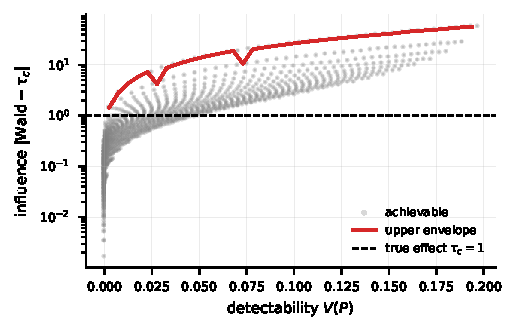
\includegraphics[width=0.52\linewidth]{figs/fig_frontier.pdf}
\caption{Pairs of $V(P)$ and $|\Wald-\tau_c|$ in the simulated family at $\mathrm{sep}=0$, sweeping $\alpha\in[0.01,0.29]$ and $\tau_f\in[1,3]$. The curve is a numerical envelope for this parameterization, not a general equilibrium frontier.}
\label{fig:frontier}
\end{figure}

Figure~\ref{fig:frontier} displays population violation against Wald distortion. These are distinct from the identified-set widths in Figure~\ref{fig:main}c. The envelope summarizes a finite parameter grid; it is not a universal feasibility boundary or an equilibrium solution. Zero-distortion points are omitted from the logarithmic vertical axis.

\section{Simulation details}\label{app:sim}

\paragraph{Generating laws.}
Assignments are independent Bernoulli$(1/2)$ draws and users are sampled
independently. Compliers have $Y(0)\sim\mathcal N(0,1)$ and
$Y(1)\sim\mathcal N(\tau_c,1)$, with $\tau_c=1$; defiers have
$Y(0)\sim\mathcal N(\mathrm{sep},1)$ and
$Y(1)\sim\mathcal N(\mathrm{sep}+\tau_f,1)$. Always-takers have
$Y(1)\sim\mathcal N(0.5,1)$ and never-takers $Y(0)\sim\mathcal N(-0.5,1)$.
Their other potential outcomes do not enter the observables. Along the share
sweeps, $\Prob(T=c)=0.30$ and $\Prob(T=a)=0.25$ stay fixed, while
$\Prob(T=n)=0.45-\alpha$. These are comparisons across DGPs, not a model of
which existing users are recruited. Unless varied explicitly, $\tau_f=\tau_c$.

\paragraph{Raw outcomes and discretization.}
Population $V(P)$ and Wald values refer to the original outcome laws.
For testing and identified sets, outcomes are winsorized to $[-6,9]$ and
mapped to $K=12$ equal-width cells (the extreme cells absorb both tails).
Let $Q(Y)$ be the cell midpoint and $P_Q$ the law of $(Z,D,Q(Y))$. Then
\[
V_Q:=V(P_Q)=\max_{d\in\{0,1\}}\sum_{k=1}^K[S_d(B_k)]_+\le V(P).
\]
Refining a partition weakly increases $V_Q$; the histogram plug-in is upward
biased for $V_Q$ by convexity, conditional on nonempty arms. Its bias relative
to the unrestricted $V(P)$ has no fixed sign. A test of these cells can miss
violations within cells. The binary simulations use their two exact cells.

\paragraph{Identified-set calculation.}
The plotted effect is $\tau_c^Q=\E[Q(Y(1))-Q(Y(0))\mid T=c]$.
Write $\theta_{tdk}=\Prob(T=t,Q(Y(d))=q_k)$. Feasible nonnegative arrays match
all four observed sub-distributions cell by cell, have equal type mass across
$d$, and total mass one. Minimize and maximize
\[
\frac{\sum_k q_k(\theta_{c1k}-\theta_{c0k})}{\sum_k\theta_{c1k}}
\]
over this set with positive complier mass. The Charnes--Cooper substitution
$s=1/\sum_k\theta_{c1k}$, $x=s\theta$ makes the objective linear and replaces
$A\theta=b$ by $Ax=bs$, with $\sum_k x_{c1k}=1$.
These are sharp population bounds for the midpoint-coded outcome, up to
solver tolerance; no Gaussian restriction, known defier share, or mimicry
restriction is imposed on candidate models. The plotted designs have a
positive first stage, which bounds the denominator away from zero.
They are not sharp bounds for the original continuous-outcome LATE.

\paragraph{Test and calibration.}
Stack the $2K$ moments $g=(m_{10}-m_{11},m_{01}-m_{00})$ on the fixed cells.
For each unit define $u_{id}=(\mathbf1\{D_i=d,Y_i\in B_k\})_{k=1}^K$
and the signed cell vector $h_i=(u_{i1}^{\mathsf T},-u_{i0}^{\mathsf T})^{\mathsf T}$.
Then $\hat g=\bar h_0-\bar h_1$, with
plug-in covariance $\widehat\Sigma_0/n_0+\widehat\Sigma_1/n_1$.
The statistic is $\max_j\hat g_j/\widehat{\mathrm{se}}_j$; its critical value
is the $0.95$ quantile of the maximum of a zero-mean Gaussian with the plug-in
correlation matrix. Zero-variance nonpositive moments are omitted; a positive
zero-variance moment triggers rejection. Setting null means to zero is least
favourable. For a fixed partition, independent sampling, nonvanishing arm
shares, and positive population variances for retained moments, this provides
pointwise asymptotic size control as sample size and the number of Gaussian draws grow.
It is not an exact finite-sample or uniformly valid sparse-cell test.
Runs use $400$ replications and $1000$ Gaussian draws per replication, with
seeds fixed in the scripts. The full run uses only CPU computation and NumPy,
SciPy, and Matplotlib.

\newpage
\section*{NeurIPS Paper Checklist}




\begin{enumerate}

\item {\bf Claims}
    \item[] Question: Do the main claims made in the abstract and introduction accurately reflect the paper's contributions and scope?
    \item[] Answer: \answerYes{}
    \item[] Justification: The abstract and introduction state that Theorem 1 restates a known bound (Richardson and Robins 2010; Noack 2021; K\'edagni, Wu and Cui 2025) and locate the contribution in the audit interpretation and numerical investigation using attributed identification results. Corollary 2 describes measure domination; Lemma 3 is explicitly credited as a known decomposition. Finding 1 concerns midpoint-coded outcomes, and Appendix C includes robustness and boundary-null diagnostics. Simulation findings are not presented as general theorems.
    \item[] Guidelines:
    \begin{itemize}
        \item The answer \answerNA{} means that the abstract and introduction do not include the claims made in the paper.
        \item The abstract and/or introduction should clearly state the claims made, including the contributions made in the paper and important assumptions and limitations. A \answerNo{} or \answerNA{} answer to this question will not be perceived well by the reviewers. 
        \item The claims made should match theoretical and experimental results, and reflect how much the results can be expected to generalize to other settings. 
        \item It is fine to include aspirational goals as motivation as long as it is clear that these goals are not attained by the paper. 
    \end{itemize}

\item {\bf Limitations}
    \item[] Question: Does the paper discuss the limitations of the work performed by the authors?
    \item[] Answer: \answerYes{}
    \item[] Justification: Section~6 and Appendix D distinguish defiance from coordination and from exclusion failure, state that rejection rates rely on a fixed partition and an asymptotic approximation, and note that no auditor--collective equilibrium is solved. Appendix C reports robustness to the outcome law, the partition, partial participation, idiosyncratic defiers, and a direct effect of the encouragement.
    \item[] Guidelines:
    \begin{itemize}
        \item The answer \answerNA{} means that the paper has no limitation while the answer \answerNo{} means that the paper has limitations, but those are not discussed in the paper. 
        \item The authors are encouraged to create a separate ``Limitations'' section in their paper.
        \item The paper should point out any strong assumptions and how robust the results are to violations of these assumptions (e.g., independence assumptions, noiseless settings, model well-specification, asymptotic approximations only holding locally). The authors should reflect on how these assumptions might be violated in practice and what the implications would be.
        \item The authors should reflect on the scope of the claims made, e.g., if the approach was only tested on a few datasets or with a few runs. In general, empirical results often depend on implicit assumptions, which should be articulated.
        \item The authors should reflect on the factors that influence the performance of the approach. For example, a facial recognition algorithm may perform poorly when image resolution is low or images are taken in low lighting. Or a speech-to-text system might not be used reliably to provide closed captions for online lectures because it fails to handle technical jargon.
        \item The authors should discuss the computational efficiency of the proposed algorithms and how they scale with dataset size.
        \item If applicable, the authors should discuss possible limitations of their approach to address problems of privacy and fairness.
        \item While the authors might fear that complete honesty about limitations might be used by reviewers as grounds for rejection, a worse outcome might be that reviewers discover limitations that aren't acknowledged in the paper. The authors should use their best judgment and recognize that individual actions in favor of transparency play an important role in developing norms that preserve the integrity of the community. Reviewers will be specifically instructed to not penalize honesty concerning limitations.
    \end{itemize}

\item {\bf Theory assumptions and proofs}
    \item[] Question: For each theoretical result, does the paper provide the full set of assumptions and a complete (and correct) proof?
    \item[] Answer: \answerYes{}
    \item[] Justification: Assumptions 1 and 2 are stated formally and monotonicity is explicitly not imposed. Theorem 1 is proved in full in Appendix A, including the attainment direction and an explicit note on why the argument is not circular. Corollary 2 and Lemma 3 have short proofs given inline; Lemma 3 is a known formula and is attributed to Angrist, Imbens and Rubin (1996) and Noack (2021). Theorem 1 is additionally verified numerically against an independent linear program over 30 data-generating processes (maximum discrepancy $8.3\times10^{-8}$).
    \item[] Guidelines:
    \begin{itemize}
        \item The answer \answerNA{} means that the paper does not include theoretical results. 
        \item All the theorems, formulas, and proofs in the paper should be numbered and cross-referenced.
        \item All assumptions should be clearly stated or referenced in the statement of any theorems.
        \item The proofs can either appear in the main paper or the supplemental material, but if they appear in the supplemental material, the authors are encouraged to provide a short proof sketch to provide intuition. 
        \item Inversely, any informal proof provided in the core of the paper should be complemented by formal proofs provided in appendix or supplemental material.
        \item Theorems and Lemmas that the proof relies upon should be properly referenced. 
    \end{itemize}

    \item {\bf Experimental result reproducibility}
    \item[] Question: Does the paper fully disclose all the information needed to reproduce the main experimental results of the paper to the extent that it affects the main claims and/or conclusions of the paper (regardless of whether the code and data are provided or not)?
    \item[] Answer: \answerYes{}
    \item[] Justification: All experiments are simulations with no external data. The code has two entry points: \texttt{run\_experiments.py} regenerates every figure and number of the main text and \texttt{robustness.py} regenerates Appendix C and the worked example of Appendix B, with seeds fixed in the scripts. Appendices C and G give the full parameterization.
    \item[] Guidelines:
    \begin{itemize}
        \item The answer \answerNA{} means that the paper does not include experiments.
        \item If the paper includes experiments, a \answerNo{} answer to this question will not be perceived well by the reviewers: Making the paper reproducible is important, regardless of whether the code and data are provided or not.
        \item If the contribution is a dataset and\slash or model, the authors should describe the steps taken to make their results reproducible or verifiable. 
        \item Depending on the contribution, reproducibility can be accomplished in various ways. For example, if the contribution is a novel architecture, describing the architecture fully might suffice, or if the contribution is a specific model and empirical evaluation, it may be necessary to either make it possible for others to replicate the model with the same dataset, or provide access to the model. In general. releasing code and data is often one good way to accomplish this, but reproducibility can also be provided via detailed instructions for how to replicate the results, access to a hosted model (e.g., in the case of a large language model), releasing of a model checkpoint, or other means that are appropriate to the research performed.
        \item While NeurIPS does not require releasing code, the conference does require all submissions to provide some reasonable avenue for reproducibility, which may depend on the nature of the contribution. For example
        \begin{enumerate}
            \item If the contribution is primarily a new algorithm, the paper should make it clear how to reproduce that algorithm.
            \item If the contribution is primarily a new model architecture, the paper should describe the architecture clearly and fully.
            \item If the contribution is a new model (e.g., a large language model), then there should either be a way to access this model for reproducing the results or a way to reproduce the model (e.g., with an open-source dataset or instructions for how to construct the dataset).
            \item We recognize that reproducibility may be tricky in some cases, in which case authors are welcome to describe the particular way they provide for reproducibility. In the case of closed-source models, it may be that access to the model is limited in some way (e.g., to registered users), but it should be possible for other researchers to have some path to reproducing or verifying the results.
        \end{enumerate}
    \end{itemize}


\item {\bf Open access to data and code}
    \item[] Question: Does the paper provide open access to the data and code, with sufficient instructions to faithfully reproduce the main experimental results, as described in supplemental material?
    \item[] Answer: \answerYes{}
    \item[] Justification: The complete simulation and audit code is distributed with the paper with a \texttt{requirements.txt} and a README describing how to run it. No data are required: all outcomes are generated from the models in Appendices C and G.
    \item[] Guidelines:
    \begin{itemize}
        \item The answer \answerNA{} means that paper does not include experiments requiring code.
        \item Please see the NeurIPS code and data submission guidelines (\url{https://neurips.cc/public/guides/CodeSubmissionPolicy}) for more details.
        \item While we encourage the release of code and data, we understand that this might not be possible, so \answerNo{} is an acceptable answer. Papers cannot be rejected simply for not including code, unless this is central to the contribution (e.g., for a new open-source benchmark).
        \item The instructions should contain the exact command and environment needed to run to reproduce the results. See the NeurIPS code and data submission guidelines (\url{https://neurips.cc/public/guides/CodeSubmissionPolicy}) for more details.
        \item The authors should provide instructions on data access and preparation, including how to access the raw data, preprocessed data, intermediate data, and generated data, etc.
        \item The authors should provide scripts to reproduce all experimental results for the new proposed method and baselines. If only a subset of experiments are reproducible, they should state which ones are omitted from the script and why.
        \item At submission time, to preserve anonymity, the authors should release anonymized versions (if applicable).
        \item Providing as much information as possible in supplemental material (appended to the paper) is recommended, but including URLs to data and code is permitted.
    \end{itemize}


\item {\bf Experimental setting/details}
    \item[] Question: Does the paper specify all the training and test details (e.g., data splits, hyperparameters, how they were chosen, type of optimizer) necessary to understand the results?
    \item[] Answer: \answerYes{}
    \item[] Justification: Appendix G specifies outcome distributions, shares, winsorization, 12 cells, and the exact Charnes--Cooper ratio program; Appendix C specifies the alternative outcome laws and scenarios. Section~5 and Appendix G specify 400 replications, 1000 Gaussian calibration draws, and nominal level $0.05$.
    \item[] Guidelines:
    \begin{itemize}
        \item The answer \answerNA{} means that the paper does not include experiments.
        \item The experimental setting should be presented in the core of the paper to a level of detail that is necessary to appreciate the results and make sense of them.
        \item The full details can be provided either with the code, in appendix, or as supplemental material.
    \end{itemize}

\item {\bf Experiment statistical significance}
    \item[] Question: Does the paper report error bars suitably and correctly defined or other appropriate information about the statistical significance of the experiments?
    \item[] Answer: \answerYes{}
    \item[] Justification: Rejection rates average 400 independent replications, so their Monte Carlo standard error is at most $0.025$. Each critical value uses 1000 draws from a plug-in least-favourable Gaussian law at level $0.05$; population quantities and discretized LP endpoints are deterministic.
    \item[] Guidelines:
    \begin{itemize}
        \item The answer \answerNA{} means that the paper does not include experiments.
        \item The authors should answer \answerYes{} if the results are accompanied by error bars, confidence intervals, or statistical significance tests, at least for the experiments that support the main claims of the paper.
        \item The factors of variability that the error bars are capturing should be clearly stated (for example, train/test split, initialization, random drawing of some parameter, or overall run with given experimental conditions).
        \item The method for calculating the error bars should be explained (closed form formula, call to a library function, bootstrap, etc.)
        \item The assumptions made should be given (e.g., Normally distributed errors).
        \item It should be clear whether the error bar is the standard deviation or the standard error of the mean.
        \item It is OK to report 1-sigma error bars, but one should state it. The authors should preferably report a 2-sigma error bar than state that they have a 96\% CI, if the hypothesis of Normality of errors is not verified.
        \item For asymmetric distributions, the authors should be careful not to show in tables or figures symmetric error bars that would yield results that are out of range (e.g., negative error rates).
        \item If error bars are reported in tables or plots, the authors should explain in the text how they were calculated and reference the corresponding figures or tables in the text.
    \end{itemize}

\item {\bf Experiments compute resources}
    \item[] Question: For each experiment, does the paper provide sufficient information on the computer resources (type of compute workers, memory, time of execution) needed to reproduce the experiments?
    \item[] Answer: \answerYes{}
    \item[] Justification: The full verification runs took approximately 85 seconds for the main script and 47 seconds for the robustness script on a laptop using CPU computation; runtime varies by system. No GPU is used; dependencies are NumPy, SciPy and Matplotlib.
    \item[] Guidelines:
    \begin{itemize}
        \item The answer \answerNA{} means that the paper does not include experiments.
        \item The paper should indicate the type of compute workers CPU or GPU, internal cluster, or cloud provider, including relevant memory and storage.
        \item The paper should provide the amount of compute required for each of the individual experimental runs as well as estimate the total compute. 
        \item The paper should disclose whether the full research project required more compute than the experiments reported in the paper (e.g., preliminary or failed experiments that didn't make it into the paper). 
    \end{itemize}
    
\item {\bf Code of ethics}
    \item[] Question: Does the research conducted in the paper conform, in every respect, with the NeurIPS Code of Ethics \url{https://neurips.cc/public/EthicsGuidelines}?
    \item[] Answer: \answerYes{}
    \item[] Justification: The research conforms to the NeurIPS Code of Ethics. It involves no human subjects, no personal data and no released models.
    \item[] Guidelines:
    \begin{itemize}
        \item The answer \answerNA{} means that the authors have not reviewed the NeurIPS Code of Ethics.
        \item If the authors answer \answerNo, they should explain the special circumstances that require a deviation from the Code of Ethics.
        \item The authors should make sure to preserve anonymity (e.g., if there is a special consideration due to laws or regulations in their jurisdiction).
    \end{itemize}


\item {\bf Broader impacts}
    \item[] Question: Does the paper discuss both potential positive societal impacts and negative societal impacts of the work performed?
    \item[] Answer: \answerYes{}
    \item[] Justification: Corollary 2 is dual-use because it characterizes when the population inequalities have no power against defiance. Appendix E explains why non-rejection is not evidence of validity and why first-stage reporting is complementary but not a complete mitigation.
    \item[] Guidelines:
    \begin{itemize}
        \item The answer \answerNA{} means that there is no societal impact of the work performed.
        \item If the authors answer \answerNA{} or \answerNo, they should explain why their work has no societal impact or why the paper does not address societal impact.
        \item Examples of negative societal impacts include potential malicious or unintended uses (e.g., disinformation, generating fake profiles, surveillance), fairness considerations (e.g., deployment of technologies that could make decisions that unfairly impact specific groups), privacy considerations, and security considerations.
        \item The conference expects that many papers will be foundational research and not tied to particular applications, let alone deployments. However, if there is a direct path to any negative applications, the authors should point it out. For example, it is legitimate to point out that an improvement in the quality of generative models could be used to generate Deepfakes for disinformation. On the other hand, it is not needed to point out that a generic algorithm for optimizing neural networks could enable people to train models that generate Deepfakes faster.
        \item The authors should consider possible harms that could arise when the technology is being used as intended and functioning correctly, harms that could arise when the technology is being used as intended but gives incorrect results, and harms following from (intentional or unintentional) misuse of the technology.
        \item If there are negative societal impacts, the authors could also discuss possible mitigation strategies (e.g., gated release of models, providing defenses in addition to attacks, mechanisms for monitoring misuse, mechanisms to monitor how a system learns from feedback over time, improving the efficiency and accessibility of ML).
    \end{itemize}
    
\item {\bf Safeguards}
    \item[] Question: Does the paper describe safeguards that have been put in place for responsible release of data or models that have a high risk for misuse (e.g., pre-trained language models, image generators, or scraped datasets)?
    \item[] Answer: \answerNA{}
    \item[] Justification: No data or models are released, so there is no artifact carrying a misuse risk requiring access controls. The dual-use consideration raised by our evasion characterization is discussed under broader impacts rather than mitigated by safeguards, since the relevant content is a mathematical condition rather than a released capability.
    \item[] Guidelines:
    \begin{itemize}
        \item The answer \answerNA{} means that the paper poses no such risks.
        \item Released models that have a high risk for misuse or dual-use should be released with necessary safeguards to allow for controlled use of the model, for example by requiring that users adhere to usage guidelines or restrictions to access the model or implementing safety filters. 
        \item Datasets that have been scraped from the Internet could pose safety risks. The authors should describe how they avoided releasing unsafe images.
        \item We recognize that providing effective safeguards is challenging, and many papers do not require this, but we encourage authors to take this into account and make a best faith effort.
    \end{itemize}

\item {\bf Licenses for existing assets}
    \item[] Question: Are the creators or original owners of assets (e.g., code, data, models), used in the paper, properly credited and are the license and terms of use explicitly mentioned and properly respected?
    \item[] Answer: \answerNA{}
    \item[] Justification: No third-party datasets, models or scraped content are used. The work depends only on standard open-source scientific Python libraries (NumPy, SciPy, Matplotlib), which are recorded in \texttt{requirements.txt}.
    \item[] Guidelines:
    \begin{itemize}
        \item The answer \answerNA{} means that the paper does not use existing assets.
        \item The authors should cite the original paper that produced the code package or dataset.
        \item The authors should state which version of the asset is used and, if possible, include a URL.
        \item The name of the license (e.g., CC-BY 4.0) should be included for each asset.
        \item For scraped data from a particular source (e.g., website), the copyright and terms of service of that source should be provided.
        \item If assets are released, the license, copyright information, and terms of use in the package should be provided. For popular datasets, \url{paperswithcode.com/datasets} has curated licenses for some datasets. Their licensing guide can help determine the license of a dataset.
        \item For existing datasets that are re-packaged, both the original license and the license of the derived asset (if it has changed) should be provided.
        \item If this information is not available online, the authors are encouraged to reach out to the asset's creators.
    \end{itemize}

\item {\bf New assets}
    \item[] Question: Are new assets introduced in the paper well documented and is the documentation provided alongside the assets?
    \item[] Answer: \answerYes{}
    \item[] Justification: The new asset is the simulation and audit code released in the supplementary material. It is documented by a README covering the claims it reproduces, the entry point, runtime and dependencies, and by module-level and function-level docstrings stating the estimands, the distinction between population and partition bounds, and the limitations of the asymptotic test. Thirteen regression tests cover scientific identities and numerical edge cases.
    \item[] Guidelines:
    \begin{itemize}
        \item The answer \answerNA{} means that the paper does not release new assets.
        \item Researchers should communicate the details of the dataset\slash code\slash model as part of their submissions via structured templates. This includes details about training, license, limitations, etc. 
        \item The paper should discuss whether and how consent was obtained from people whose asset is used.
        \item At submission time, remember to anonymize your assets (if applicable). You can either create an anonymized URL or include an anonymized zip file.
    \end{itemize}

\item {\bf Crowdsourcing and research with human subjects}
    \item[] Question: For crowdsourcing experiments and research with human subjects, does the paper include the full text of instructions given to participants and screenshots, if applicable, as well as details about compensation (if any)? 
    \item[] Answer: \answerNA{}
    \item[] Justification: The paper involves no crowdsourcing and no research with human subjects. All users in the paper are simulated draws from the models in Appendices C and G.
    \item[] Guidelines:
    \begin{itemize}
        \item The answer \answerNA{} means that the paper does not involve crowdsourcing nor research with human subjects.
        \item Including this information in the supplemental material is fine, but if the main contribution of the paper involves human subjects, then as much detail as possible should be included in the main paper. 
        \item According to the NeurIPS Code of Ethics, workers involved in data collection, curation, or other labor should be paid at least the minimum wage in the country of the data collector. 
    \end{itemize}

\item {\bf Institutional review board (IRB) approvals or equivalent for research with human subjects}
    \item[] Question: Does the paper describe potential risks incurred by study participants, whether such risks were disclosed to the subjects, and whether Institutional Review Board (IRB) approvals (or an equivalent approval/review based on the requirements of your country or institution) were obtained?
    \item[] Answer: \answerNA{}
    \item[] Justification: No research with human subjects was conducted, so no IRB review or equivalent was required.
    \item[] Guidelines:
    \begin{itemize}
        \item The answer \answerNA{} means that the paper does not involve crowdsourcing nor research with human subjects.
        \item Depending on the country in which research is conducted, IRB approval (or equivalent) may be required for any human subjects research. If you obtained IRB approval, you should clearly state this in the paper. 
        \item We recognize that the procedures for this may vary significantly between institutions and locations, and we expect authors to adhere to the NeurIPS Code of Ethics and the guidelines for their institution. 
        \item For initial submissions, do not include any information that would break anonymity (if applicable), such as the institution conducting the review.
    \end{itemize}

\item {\bf Declaration of LLM usage}
    \item[] Question: Does the paper describe the usage of LLMs if it is an important, original, or non-standard component of the core methods in this research? Note that if the LLM is used only for writing, editing, or formatting purposes and does \emph{not} impact the core methodology, scientific rigor, or originality of the research, declaration is not required.
    %this research? 
    \item[] Answer: \answerNA{}
    \item[] Justification: No LLM is an important, original, or non-standard component of the theory or simulation.
    \item[] Guidelines:
    \begin{itemize}
        \item The answer \answerNA{} means that the core method development in this research does not involve LLMs as any important, original, or non-standard components.
        \item Please refer to our LLM policy in the NeurIPS handbook for what should or should not be described.
    \end{itemize}

\end{enumerate}


\end{document}
